\chapter{Introduction}
\label{chap:thesis-intro}

Digital music builds on a rich music tradition in the acoustic realm, but also differs from it by nature: Instead of directly reaching our ears, digital music first needs to be represented as data that a computer can process. Our listening experience depends on the quality of the representation. Design and engineering decisions lie behind the representation, from the sound wave itself---stored as a sequence of numbers---to musical structure, including melody, harmony, and rhythm. In this thesis, I introduce an automatic pitch correction algorithm for singing voice. The pitch representation in the algorithm is designed to capture the complex way we experience pitch and manipulate it when singing. This thesis work builds on studies of how physical measures of pitch, such as frequency and timbre, map to what we hear through a complex psychoacoustic process influenced by our musical upbringing. This complex process results in us either considering a note to be ``in tune'' or not.

Music making with family, friends, and the wider community is one of the universally enjoyed activities across the world. In recent years, digital options have emerged in applications such as Smule, Spotify, Cadenza, YouTube, and TikTok. These enable people to share their recordings with their peers, and provide tools for collaboration and audio processing that only exist in the digital realm. These apps use post-processing, which involves editing the track after it has been recorded to improve the quality. Automatic pitch correction to make a performance sound in tune is one type of post-processing. 

Why not just leave the recording unaltered? As anyone who has tried to photograph a beautiful landscape has experienced, capturing the natural colors, beauty, and atmosphere of a scene is challenging. Image post-processing might actually make the outcome better capture reality or, alternatively, bring to the viewer's attention aspects of the landscape that could otherwise be easily missed. In the same way, post-processing of audio can enhance the listening experience: The listener is hearing the performance through the recording and playback pipeline, outside of the original acoustic setting. A performance heard recorded versus live can be a substantially different musical experience.

The process of producing a digital recording can range from professional to recreational. Professional digital recording involves the use of professional audio-editing software, high-end microphones, and recording spaces with good acoustics, all of which require considerable time and resources. It results in a polished and high-quality result. The recreational kind often involves multipurpose recording devices such as smartphones, and typically involves little in the way of time and resources. Music apps can serve as a platform for recreational music making. Apps can provide a meaningful musical opportunity. Users of Smule, Inc, a singing app, have reported taking a ten-minute break in their workday to sing, and shared with the company how that short singing break brings them joy and reduces their stress. Without being willing to invest time and money in editing their recording or having the resources or training to do so, recreational musicians may still benefit from using post-processing tools that are built into the app. These apply automatic pitch correction or add effects such as reverb. Post-processing tools do not replace professional audio editing, but are recognized as improving the quality of the recording with remarkably little effort or cost. Although post-processing tools do not make a recording sound professional, they can make it more pleasing to a listener. A parallel can be seen when a person uses a grammar-checker to improve the quality of their writing, even when writing simple text such as an email. The ability of the grammar-checker to remove minor errors produces a more polished result, which can make a big difference, especially given the high stakes of sharing content in a recorded format.

\begin{figure}[t!]
    \centering
    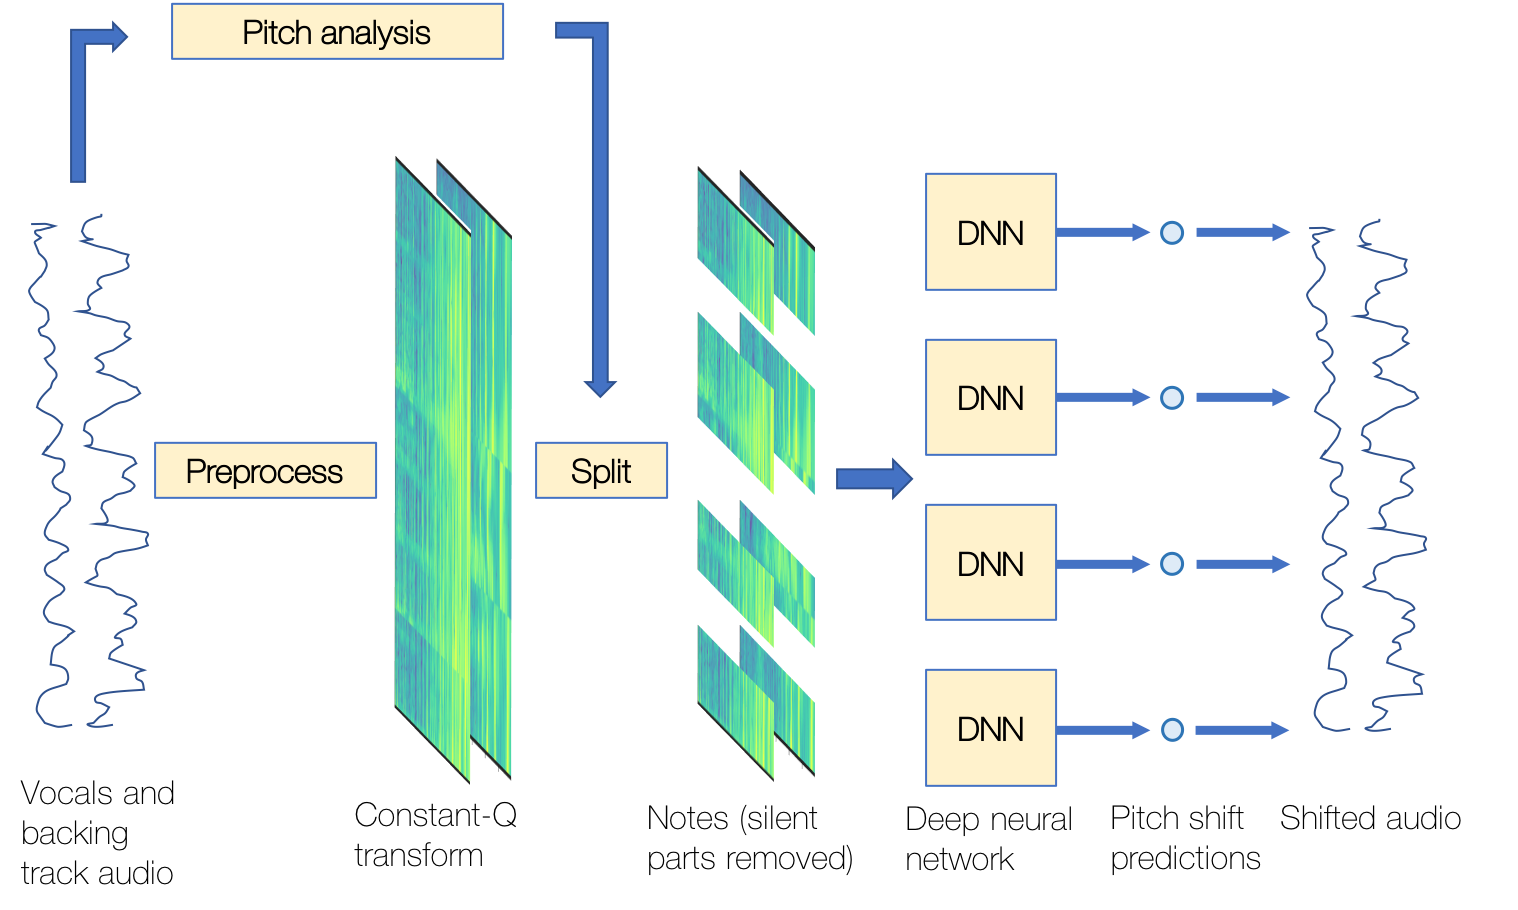
\includegraphics[width=\columnwidth]{images/program_flow_chart.png}
    \caption{Pitch correction algorithm overview. The algorithm requires audio for the vocals and backing track (also called accompaniment) on separate audio tracks. It applies the constant-Q transform to the audio to generate time-frequency representations. It then splits the data into individual notes based on the measured singing frequency. It discards silent sections in the audio. Next, for every note, it predicts a pitch correction shift using a deep neural network (DNN) trained on real-world singing examples. Finally, in the post processing phase, it applies the shifts to every note and combines them along with silent sections to construct the corrected track. }
    \label{fig:results}
\end{figure}

\section{Challenges in data-driven automatic pitch correction}

I illustrate the complexity of the task of automatic pitch correction by describing the difference between a musical score and a performance. In a musical score, a melody for singing voice is typically notated as a sequence of notes of discretized lengths and pre-defined pitches. The simplicity of the symbolic representation leaves considerable scope for variation in the singer's interpretation. Even when a vocalist follows the general contour of the score, the singing voice actually varies continuously due to expressive gestures such as pitch bending, vibrato, and other variations coming from musical tradition, personal preference, and randomness. A singer's deviation from the symbolic score is sometimes large, as described in Chapter \ref{chap:intonation}.

In existing commercial systems for automatic pitch correction, vocal track notes are typically shifted to be centered around pitches in a user-defined score, or mapped to the closest pitch among the twelve equal-tempered scale degrees (e.g., \cite{antares:2018}). This approach reliably corrects out-of-tune singing. The downside is that it also removes intentional nuances whenever pitch deviates from the symbolic score. 

The algorithm in this thesis represents pitch as a continuous parameter instead of a discretized value. This continuous representation enables it to preserve the nuanced variations of sung pitch while applying corrections. Furthermore, the algorithm makes its predictions purely on the audio content of the vocals and backing track (also called accompaniment), without relying on a musical score. This leaves room for the singer to sing a different melody, as is common when harmonizing or improvising. %, while also correcting the amount of unintended pitch shift. %It predicts corrections for these unintended deviations.%The priority is to output a result that sounds natural and aesthetically pleasing. If this is not the case, the user will prefer the unprocessed recording. 

Making a singer's pitch track sound more in tune without relying on a symbolic score is not straightforward. The algorithm must behave like a human listener with a moderate level of musical understanding. Such a listener can often detect the out-of-tune notes and predict the amount and direction of the pitch shift required to bring the note back in tune, all without requiring access to the score. The algorithm in this thesis uses a Deep Neural Network (\gls{dnn}) to make predictions. The \gls{dnn} is trained on real-world singing examples, from which it learns patterns of intonation that help it make accurate predictions.

Training data for automatic pitch correction is hard to find. The first challenge involves collecting examples of in-tune singing. Publicly available datasets typically mix performances of all levels of singing, in tune and out of tune. The in-tune recordings need to be extracted to form a smaller training dataset. The second challenge---if training the \gls{dnn} in a supervised manner---is to design data pairs where the input is out of tune, the target is in tune, but the signals are otherwise identical. Such pairs don't occur naturally, making data synthesis a viable approach. Synthesizing out-of-tune singing from an in-tune performance, however, requires defining a de-tuning algorithm, which is a challenge in itself. Chapters \ref{chap:intonation} and \ref{chap:tech-background} illustrate the difficulty of representing pitch as a set of features that can be measured and manipulated. Chapter \ref{chap:thesis-autotuner} delves into the numerous decisions around feature design. 

\section{Overview}
The algorithm introduced in this thesis predicts pitch corrections of solo singing performances in a data-driven manner. It predicts note-wise pitch shifts from the relationship between the respective spectrograms of the singing and backing track. It outputs the amount and direction of the pitch shift expected to bring the note back in tune. The pitch shift predictions are constant by note, and continuous in frequency. In post-processing, the algorithm applies the shifts to each note, as shown in Figure \ref{fig:results}. It does not require access to the musical score, which makes it usable even when the singer improvises or harmonizes in a performance.

The algorithm is designed to utilize information similarly to the human ear, basing corrections on information found in the audio, such as the level of perceived musical harmony and context in time. It is a \gls{dnn} trained on patterns in real-world singing examples from a dataset of 4,702 amateur karaoke performances selected for good intonation \cite{wager2018intonation}. The model is trained on both incorrect intonation, for which it learns a correction, and intentional pitch variation, which it learns to preserve. The design of the algorithm is based on the empirically derived conceptualization of musical intonation described in Section \ref{sec:empirical}. Given its flexibility and preservation of nuance, it is adaptable to different musical traditions, regardless of the scales and pitch-related practices used in these traditions. It is a step towards a model-free automatic pitch correction system, the use of which is justified in Chapter \ref{chap:tech-background}. 

The proposed \gls{dnn} architecture includes convolutional layers for feature extraction followed by Gated Recurrent Units (\gls{gru}s) for sequential processing. The algorithm shows promising performance on the real-world score-free singing pitch correction task. To the best of my knowledge, this is the first data-driven approach to correcting singing voice pitch based on the harmonic content of the backing track.

\section{Scope and limitations}
The algorithm---designed for amateur singing---is intended for situations where a singer wishes to apply simple post-processing---for example, on their smartphone---without using professional audio-editing software. It requires that the vocals and backing track be separate, and for the vocals to be monophonic and free of noise. The current algorithm is limited to post-processing: Adapting it for real-time processing is left to future work.

The assumptions on which the algorithm is based are strong and might not be accurate. First, the backing track is assumed to have clearly identifiable pitches---a chord progression---that serves as a reference for the vocals. Second, only past and current musical content is needed for making a prediction. the \gls{dnn} processes a performance as a sequence in time, and does not access data from the future. Third, each note is corrected by a constant amount, and this is assumed to produce an accurate sounding result. Fourth, the dataset used to train the algorithm is assumed to be in-tune enough for this prototype, despite consisting of amateur singing, which sounds different from professional singing. %tune


\section{Contributions}
Contributions in this thesis include:
\begin{itemize}
    \item A data-driven algorithm for predicting pitch corrections directly based on the time-frequency content of the vocals and backing tracks instead of based on a symbolic music score.
    \item Continuous representation of pitch, which enables the algorithm to preserve pitch nuances, and to incorporate concepts from psychoacoustics, physics of sound, and cultural practices regarding musical intonation.
    \item A technique for generating pairs of training examples where one is in tune and the other is out of tune. This involves de-tuning in-tune performances to synthesize out-of-tune singing. De-tuning is based on random sampling from a \gls{hmm} \cite{rabiner1989tutorial}.
    \item Adaptability to any musical culture for which training data is available.
    \item An adaptation of a \gls{dnn} architecture for pitch detection---including convolutional and Gated Recurrent Unit \cite{chung2014empirical} layers---to the task of automatic pitch correction. The convolutional layers are used to extract features, while the \gls{gru} layers process the music signal sequentially.
    \item The ``Intonation'' dataset of in-tune singing performances, including the time-frequency magnitude transformation of the backing tracks and other metadata.
    \item A commentary on transforming this algorithm into a system that is usable in practice, even given the fact that not all of its corrections will result in higher accuracy.
    \item A small-scale subjective listening test, where the deep pitch correction network is shown to provide convincing adjustments when the backing track includes clear reference pitches.
\end{itemize}

\section{Outline}
\textbf{Chapter \ref{chap:intonation}} provides a musical background for the algorithm design, placing its development in the context of the discussion of musical intonation that has occurred over millenia. It surveys two standard conceptualizations of musical intonation, relevant definitions, and describes musical cultures that use intonation in different ways. This chapter also describes Antares Auto-Tune, one of the music-industry standards for pitch correction, discussing its advantages and disadvantages, and what can be learned from it when developing a data-driven pitch-correction algorithm. 

\textbf{Chapter \ref{chap:tech-background}} discusses the technical background. It provides an overview of music representation in software and compares model-driven approaches to data-driven approaches, including how they affect control, interpretability, and expressivity of the programs. It concludes with reasons behind the choice of a deep neural network for the task of automatic pitch correction.

\textbf{Chapter \ref{chap:thesis-autotuner}} provides a technical presentation of the proposed algorithm. It starts with an overview of related work in music information retrieval, deep learning, and audio signal processing. It then describes in detail the proposed algorithm. This includes note boundary detection techniques, pitch de-tuning techniques, model architecture choices, and the experimental configuration.

\textbf{Chapter \ref{chap:thesis-damp}} describes how we collected the ``Intonation'' dataset and details about the dataset. It indicates how the clustering technique used to collect the data can be used to generate datasets for other tasks where the target is subjective---as it is in the case of musical intonation. It also describes shortcomings related to genre bias in the current dataset, and how this issue can be fixed in future work.

\textbf{Chapter \ref{chap:results}} describes results both on the synthesized test set and the real-world dataset. It includes a comparison of the results using pitch deviation histograms. It also includes a comparison of the pitch behavior in the various datasets used in this thesis work. The quantitative analysis is followed by a qualitative listening test that provides insights into the way the model works. The analysis indicates that the proposed approach is more reliable than a conceptually and computationally simple baseline. It also indicates that the proposed approach effectively utilizes pitch content in the backing track.

\textbf{Chapter \ref{chap:conclusion}} concludes the thesis. It summarizes the proposed automatic pitch correction algorithm, describes its current limitations, and how these might be addressed in future work. It places this thesis work into the broader context of music information retrieval.
